% !TEX root = ./CV_Lasse_D_Skaalum.tex

%============================================================================%
%
%	DOCUMENT DEFINITION
%
%============================================================================%

%we use article class because we want to fully customize the page and don't use a cv template
\documentclass[10pt,A4]{article}	

% Skabelon: https://www.overleaf.com/latex/templates/jan-kusters-left-sidebar-cv/tmmnhrkcmpgv

%----------------------------------------------------------------------------------------
%	ENCODING
%----------------------------------------------------------------------------------------

% we use utf8 since we want to build from any machine
\usepackage[utf8]{inputenc}

%----------------------------------------------------------------------------------------
%	LOGIC
%----------------------------------------------------------------------------------------

% provides \isempty test
\usepackage{xstring, xifthen}

%----------------------------------------------------------------------------------------
%	FONT BASICS
%----------------------------------------------------------------------------------------

% some tex-live fonts - choose your own

%\usepackage[defaultsans]{droidsans}
%\usepackage[default]{comfortaa}
%\usepackage{cmbright}
\usepackage[default]{raleway}
%\usepackage{fetamont}
%\usepackage[default]{gillius}
%\usepackage[light,math]{iwona}
%\usepackage[thin]{roboto} 

% set font default
\renewcommand*\familydefault{\sfdefault} 	
\usepackage[T1]{fontenc}

% more font size definitions
\usepackage{moresize}
% to be able to use ½
\usepackage{textcomp}

%----------------------------------------------------------------------------------------
%	FONT AWESOME ICONS
%---------------------------------------------------------------------------------------- 

% include the fontawesome icon set
\usepackage{fontawesome}

% use to vertically center content
% credits to: http://tex.stackexchange.com/questions/7219/how-to-vertically-center-two-images-next-to-each-other
\newcommand{\vcenteredinclude}[1]{\begingroup
\setbox0=\hbox{\includegraphics{#1}}%
\parbox{\wd0}{\box0}\endgroup}

% use to vertically center content
% credits to: http://tex.stackexchange.com/questions/7219/how-to-vertically-center-two-images-next-to-each-other
\newcommand*{\vcenteredhbox}[1]{\begingroup
\setbox0=\hbox{#1}\parbox{\wd0}{\box0}\endgroup}

% icon shortcut
\newcommand{\icon}[3] { 							
	\makebox(#2, #2){\textcolor{maincol}{\csname fa#1\endcsname}}
}	

% icon with text shortcut
\newcommand{\icontext}[4]{ 						
	\vcenteredhbox{\icon{#1}{#2}{#3}}  \hspace{2pt}  \parbox{0.9\mpwidth}{\textcolor{#4}{#3}}
}

% icon with website url
\newcommand{\iconhref}[5]{ 						
    \vcenteredhbox{\icon{#1}{#2}{#5}}  \hspace{2pt} \href{#4}{\textcolor{#5}{#3}}
}

% icon with email link
\newcommand{\iconemail}[4]{ 						
    \vcenteredhbox{\icon{#1}{#2}{#4}}  \hspace{2pt} \href{mailto:#3}{\textcolor{#4}{#3}}
}

%----------------------------------------------------------------------------------------
%	PAGE LAYOUT  DEFINITIONS
%----------------------------------------------------------------------------------------

% page outer frames (debug-only)
% \usepackage{showframe}		

% we use paracol to display breakable two columns
\usepackage{paracol}

% define page styles using geometry
\usepackage[a4paper]{geometry}

% remove all possible margins
\geometry{top=1cm, bottom=1cm, left=1cm, right=1.5cm}

% fixes a weird bug where items in itemize environments would break the margin
\usepackage{enumitem}
\setlist{rightmargin=2.5mm}

\usepackage{fancyhdr}
\pagestyle{empty}

% space between header and content
% \setlength{\headheight}{0pt}

% indentation is zero
\setlength{\parindent}{0mm}

% Hyphenation
\hyphenation{In-te-res-se-e-le-ment}

%----------------------------------------------------------------------------------------
%	TABLE /ARRAY DEFINITIONS
%---------------------------------------------------------------------------------------- 

% extended aligning of tabular cells
\usepackage{array}

% custom column right-align with fixed width
% use like p{size} but via x{size}
\newcolumntype{x}[1]{%
>{\raggedleft\hspace{0pt}}p{#1}}%


%----------------------------------------------------------------------------------------
%	GRAPHICS DEFINITIONS
%---------------------------------------------------------------------------------------- 

%for header image
\usepackage{graphicx}

% use this for floating figures
% \usepackage{wrapfig}
% \usepackage{float}
% \floatstyle{boxed} 
% \restylefloat{figure}

%for drawing graphics		
\usepackage{tikz}				
\usetikzlibrary{shapes, backgrounds,mindmap, trees}

%----------------------------------------------------------------------------------------
%	Color DEFINITIONS
%---------------------------------------------------------------------------------------- 
\usepackage{transparent}
\usepackage{color}

% primary color
\definecolor{maincol}{RGB}{ 50, 100, 250 }

% accent color, secondary
% \definecolor{accentcol}{RGB}{ 250, 150, 10 }

% dark color
\definecolor{darkcol}{RGB}{ 70, 70, 70 }

% light color
\definecolor{lightcol}{RGB}{245,245,245}

% soft light blue color (for hyperlinks)
\definecolor{lightblue}{RGB}{51, 122, 183}

% Package for links, must be the last package used
\usepackage[hidelinks]{hyperref}
\hypersetup{colorlinks,urlcolor=lightblue} 

% returns minipage width minus two times \fboxsep
% to keep padding included in width calculations
% can also be used for other boxes / environments
\newcommand{\mpwidth}{\linewidth-\fboxsep-\fboxsep}
	


%============================================================================%
%
%	CV COMMANDS
%
%============================================================================%

%----------------------------------------------------------------------------------------
%	 CV LIST
%----------------------------------------------------------------------------------------

% renders a standard latex list but abstracts away the environment definition (begin/end)
\newcommand{\cvlist}[1] {
	\begin{itemize}{#1}\end{itemize}
}

%----------------------------------------------------------------------------------------
%	 CV TEXT
%----------------------------------------------------------------------------------------

% base class to wrap any text based stuff here. Renders like a paragraph.
% Allows complex commands to be passed, too.
% param 1: *any
\newcommand{\cvtext}[1] {
	\begin{tabular*}{1\mpwidth}{p{1\mpwidth}}
		\parbox{1\mpwidth}{#1}
	\end{tabular*}
}

%----------------------------------------------------------------------------------------
%	CV SECTION
%----------------------------------------------------------------------------------------

% Renders a a CV section headline with a nice underline in main color.
% param 1: section title
\newcommand{\cvsection}[1] {
	\vspace{14pt}
	\cvtext{
		\textbf{\huge{\textcolor{darkcol}{\uppercase{#1}}}}\\[-4pt]
		\textcolor{maincol}{ \rule{0.1\textwidth}{2pt} } \\
	}
}

%----------------------------------------------------------------------------------------
%	META SKILL
%----------------------------------------------------------------------------------------

% Renders a progress-bar to indicate a certain skill in percent.
% param 1: name of the skill / tech / etc.
% param 2: level (for example in years)
% param 3: percent, values range from 0 to 1
\newcommand{\cvskill}[3] {
	\begin{tabular*}{1\mpwidth}{p{0.72\mpwidth}  r}
 		\textcolor{black}{\textbf{#1}} & \textcolor{maincol}{#2}\\
	\end{tabular*}%
	
	\hspace{4pt}
	\begin{tikzpicture}[scale=1,rounded corners=2pt,very thin]
		\fill [lightcol] (0,0) rectangle (1\mpwidth, 0.15);
		\fill [maincol] (0,0) rectangle (#3\mpwidth, 0.15);
  	\end{tikzpicture}%
}


%----------------------------------------------------------------------------------------
%	 CV EVENT
%----------------------------------------------------------------------------------------

% Renders a table and a paragraph (cvtext) wrapped in a parbox (to ensure minimum content
% is glued together when a pagebreak appears).
% Additional Information can be passed in text or list form (or other environments).
% the work you did
% param 1: time-frame i.e. Sep 14 - Jan 15 etc.
% param 2:	 event name (job position etc.)
% param 3: Customer, Employer, Industry
% param 4: Short description
% param 5: work done (optional)
% param 6: technologies include (optional)
% param 7: achievements (optional)
\newcommand{\cvevent}[7] {
	
	% we wrap this part in a parbox, so title and description are not separated on a pagebreak
	% if you need more control on page breaks, remove the parbox
	\parbox{\mpwidth}{
		\begin{tabular*}{1\mpwidth}{p{0.72\mpwidth}  r}
	 		\textcolor{black}{\Large\textbf{#2}} & \colorbox{maincol}{\makebox[0.25\mpwidth]{\textcolor{white}{#1}}} \\
			\textcolor{maincol}{\textbf{#3}} & \\
		\end{tabular*}\\[8pt]
	
		\ifthenelse{\isempty{#4}}{}{
			\cvtext{#4}
		}
	}

	\ifthenelse{\isempty{#5}}{}{
		\vspace{1pt} %Her stod 9pt før
		{#5}
	}

	\ifthenelse{\isempty{#7}}{}{
		\vspace{1pt} %Her stod 9pt før
		\cvtext{\textbf{Resultater:}}
		{#7}
	}

	\ifthenelse{\isempty{#6}}{}{
		\vspace{1pt} %Her stod 9pt før
		\cvtext{\textbf{Involverede teknologier:}}
		{#6}
	}
	\vspace{14pt}
}

%----------------------------------------------------------------------------------------
%	 CV META EVENT
%----------------------------------------------------------------------------------------

% Renders a CV event on the sidebar
% param 1: title
% param 2: subtitle (optional)
% param 3: customer, employer, etc,. (optional)
% param 4: info text (optional)
\newcommand{\cvmetaevent}[4] {
	\textcolor{maincol} {\cvtext{\textbf{\begin{flushleft}#1\end{flushleft}}}}

	\ifthenelse{\isempty{#2}}{}{
	\textcolor{darkcol} {\cvtext{\textbf{#2}} }
	}

	\ifthenelse{\isempty{#3}}{}{
		\cvtext{{ \textcolor{darkcol} {#3} }}\\
	}

	\cvtext{#4}\\[14pt]
}

%---------------------------------------------------------------------------------------
%	QR CODE
%----------------------------------------------------------------------------------------

% Renders a qrcode image (centered, relative to the parentwidth)
% param 1: percent width, from 0 to 1
\newcommand{\cvqrcode}[1] {
	\begin{center}
        \textcolor{maincol}{Min LinkedIn}
    \end{center}
	\begin{center}
		
\includegraphics[width={#1}\mpwidth]{qrcode}
	\end{center}
}

%============================================================================%
%
%
%
%	DOCUMENT CONTENT
%
%
%
%============================================================================%
\begin{document}
\columnratio{0.32}
\setlength{\columnsep}{2.2em}
\setlength{\columnseprule}{4pt}
\colseprulecolor{lightcol}
\begin{paracol}{2}
	\begin{leftcolumn}
		%---------------------------------------------------------------------------------------
		%	META IMAGE
		%----------------------------------------------------------------------------------------
		\begin{figure}[h]
			\centering
			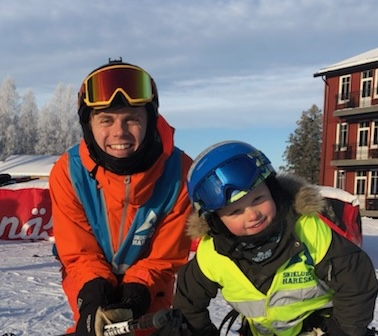
\includegraphics[width=0.93\linewidth]{ski-pb.jpg}	%trimming relative to image size and aligning "FÆRDIGHEDER" with "PROFIL"
		\end{figure}


		%---------------------------------------------------------------------------------------
		%	META SKILLS
		%----------------------------------------------------------------------------------------
		\cvsection{FÆRDIGHEDER}

		\cvskill{Undervisningserfaring}
						{} {1} \\[-2pt]

		\cvskill{Skiundervisning}
			      {40 uger} {0.8} \\[-2pt]

		\cvskill{Samarbejde}
		        {} {1} \\[-2pt]

		\cvskill{Kommunikation}
		        {} {1} \\[-2pt]

		\cvskill{Planlægning}
		        {} {0.9} \\[-2pt]

		\cvskill{Ansvarlighed}
		        {} {1} \\[-2pt]

		\cvskill{Arbejde med børn}
		        {} {1} \\[-2pt]


		\vfill\null
		\cvsection{KONTAKT}\\
		\icontext{MapMarker}{12}{\#106, Almeria E, Block C\\137 Al Mouj, Muscat, Oman}{black}\\[6pt]
		% \iconhref{MobilePhone}{12}{+45 4241 1996}{tel:+4542411996}{black}\\[6pt]
		\iconhref{MobilePhone}{12}{+968 7748 1996}{tel:+96877481996}{black}\\[6pt]
		\iconemail{Envelope}{12}{lasse@bluebirdday.dk}{black}\\[6pt]
		\iconhref{Linkedin}{12}{linkedin.com/in/lasse-skaalum}{https://www.linkedin.com/in/lasse-skaalum/}{black}\\[-12pt]

		% \vfill\null
		% \cvqrcode{0.7}

		%---------------------------------------------------------------------------------------
		%	EDUCATION
		%----------------------------------------------------------------------------------------
		\newpage
		\cvsection{UDDANNELSE}

		\cvmetaevent
		{2019 - 2022}
		{B. Sc. Software}
		{Aalborg Universitet}

		\vspace{-4em}

		% \cvmetaevent
		% {2013 - 2016}
		% {Studentereksamen (stx)}
		% {Silkeborg Gymnasium}
		% {Studerende på linjen: Bioteknologi A, Matematik A, Fysik B.\\
		% 	Tilvalgsfag: Informationstekno-logi C}

		\cvmetaevent
		{2012 - 2013}
		{Efterskole}
		{Vestbirk Musik- og Sportsefterskole\\}
		{Elev på 10. klassetrin med linjerne musik og springgymnastik.}

		% \vfill\null
		% \cvqrcode{0.7}

		%---------------------------------------------------------------------------------------
		%	CERTIFICATION
		%----------------------------------------------------------------------------------------
		% \newpage
		\cvsection{KURSER}

		\cvmetaevent
		{2019}
		{Højskoleophold}
		{Forårssemester}
		{Forårssemester på \textbf{Gerlev Idrætshøjskole} med parkour som hovedfag og springgymnastik samt windsurfing som sidefag.}

		\cvmetaevent
		{2018}
		{Skiinstruktør}
		{BSI 1}
		{To ugers skiinstruktørundervisning med \textbf{Den Danske Skiskole}.}

		% \cvmetaevent
		% {2016}
		% {Master Class Matematik}
		% {Master Class Matematik 2016}
		% {Deltog i Master Class Matematik 2016, som er et kursus arrangeret af \textbf{Sciencetalenter} for særligt talentfulde elever i 3.g.}

		\cvmetaevent
		{2015}
		{Parkourtræner}
		{DGIs parkourtræneruddannelse}
		{Modtog en uges parkour-trænerundervisning.}

		% \vfill\null
		% \cvqrcode{0.7}

		% \newpage
		% \mbox{} % hotfix to place qrcode on the bottom when there are not other elements
		% \vfill
		% \cvqrcode{0.7}

		\newpage
	\end{leftcolumn}
	\begin{rightcolumn}
		%---------------------------------------------------------------------------------------
		%	TITLE  HEADER
		%----------------------------------------------------------------------------------------
		\fcolorbox{white}{darkcol}{\begin{minipage}[c][3.5cm][c]{1\mpwidth}
				\begin {center}
				\HUGE{ \textbf{ \textcolor{white}{ \uppercase{ Lasse D. Skaalum } } } } \\[-24pt]
				\textcolor{white}{ \rule{0.1\textwidth}{1.25pt} } \\[4pt]
				\large{ \textcolor{white} {Skiglæde, skiglæde, skiglæde!} }
				\end {center}
			\end{minipage}} \\[14pt]
		\vspace{-12pt}

		\textit{Senest opdateret: \today}

		%---------------------------------------------------------------------------------------
		%	PROFILE
		%----------------------------------------------------------------------------------------
		\vspace{0.5cm}
		\emergencystretch 3em
		% Make sure no text breaks the margins
		\cvsection{PROFIL}

		\cvtext{Jeg er en entusiastisk og udadvendt skiinstruktør med 40 ugers undervisningserfaring og en passion for at skabe skiglæde og fællesskab. Jeg trives bedst i miljøer, hvor hygge, læring og gode relationer er i fokus.\\

		Med 3 års fuldtidserfaring som softwareudvikler kombineret med kontinuerlig skiundervisning og frivilligt arbejde i skiklubber, har jeg udviklet en naturlig evne til at undervise alle aldre og niveauer. Jeg skaber altid en tryg og lærerig atmosfære, hvor deltagernes udvikling står i centrum.\\

		Som jeres skiinstruktør får I en engageret og erfaren kollega, som altid prioriterer deltagernes sikkerhed og skiglæde først, og som naturligt bidrager til det positive fællesskab i jeres klub.
		}

		%----------------------------------------------------------------------------------------
		%	WORK EXPERIENCE
		%----------------------------------------------------------------------------------------
		\vfill\null
		\cvsection{ERHVERVSERFARING}

		% \cvevent
		% {Aug 24 - Sep 25}
		% {Softwarekonsulent}
		% {Trifork - Muscat}
		% {Udstationeret på Big Data projekt}
		% {\cvlist{
		% 	\item Ansvarlig for implementering af nye features, bugfixes, automatiseringer samt udskifting af fysisk hardware på en Big Data platform med yderst store datamængder.
		% 	\item Varetog en kritisk rolle for projektet i udviklings- test- og implementeringsfasen af platformen.
		% 	\item Pitchede \href{https://trifork.com/corax-ai/}{Corax AI} og \href{https://trifork.com/dataplatform/}{Corax Data} for potentielle kunder i Oman.
		% }}%Arbejdsopgaver
		% {\cvlist{
		% 	\item Spring Boot (Java), Python, Docker, Grafana, Apache Kafka, Apache Flink, Elasticsearch, JavaScript, Node.js, Ansible
		% }}%Involverede teknologier
		% {}%Resultater

		% \cvevent
		% {Jun 23 - Jul 24}
		% {Softwarekonsulent}
		% {Trifork - København}
		% {}
		% {}%Arbejdsopgaver
		% {\cvlist{
		% 	\item ASP.NET (C\#), Azure, Docker, React.js (TypeScript), Node.js, Swift
		% }}%Involverede teknologier
		% {\cvlist{
		% 	\item Forbandt SAP og MongoDB's Realm med microservices ifbm. version 3 af Banedanmarks app, Vedligehold (VHQM).
		% 	\item Stod for cloudmigreringen af Banedanmarks webapplikation, Mobile Kontrolskemaer (MKS).
		% 	\item Udviklede Speak-S for DSB - en platform som bruges til at planlægge udkald på S-Togsstationerne i Danmark.
		% }}%Resultater

		% \cvevent
		% {Sep 23 - nu}
		% {Interim CTO}
		% {DJTILBUD (deltid)}
		% {}
		% {}%Arbejdsopgaver
		% {\cvlist{
		% 	\item React.js (TypeScript), Next.js, Supabase, Grafana
		% 	}}%Involverede teknologier
		% {\cvlist{
		% 	\item Stod for at udvikle \href{https://djtilbud.dk/}{DJTILBUD}s platform fra bunden af, hvor kunder kan modtage tre tilbud fra forskellige DJs.
		% 	\item Jobsamtaler samt oplæring af udenlandske software freelancere.
		% }}%Resultater

		\cvevent
		{Feb 22 - Jun 23}
		{Teknisk Direktør \& Medstifter}
		{Instructr}
		{Instructr var en B2B SaaS-virksomhed, hvor vi byggede et white-label hybrid learning produkt til skiskoler.}
		{}%Arbejdsopgaver
		{}%Involverede teknologier
		{}%Resultater

		% \cvevent
		% {Jun 21 - Jun 22}
		% {Softwareudvikler}
		% % {Studenterprogrammør}
		% {Trifork - Aalborg}
		% {}
		% {\cvlist{
		% 		\item Domænemodellering af et HR-datasystem både i backend og på databaseniveau.
		% 		\item API design og implementering.
		% 		\item Udarbejdning af svejseremulator i Swift.
		% 	}}%Arbejdsopgaver
		% {\cvlist{
		% 		\item ASP.NET (C\#), React.js (TypeScript), React Native, MS SQL, Azure, Docker, Swift, Kotlin, Java
		% 	}}%Involverede teknologier
		% {}%Resultater

		\cvevent
		{Maj 21 - Jun 22}
		{Mentor}
		{Aalborg Universitet}
		{Mentor for en softwareenginiørstuderende. Jeg hjalp den studerende med at forstå stoffet i kurserne samt at finde sig til rette socialt.}
		{}%Arbejdsopgaver
		{}%Involverede teknologier
		{}%Resultater

		\cvevent
		{Sep 20 - Jun 21}
		{Hjælpelærer}
		{Aalborg Universitet}
		{Hjælpelærer i fagene \textbf{Imperativ Programmering} og \textbf{Algoritmer og Datastrukturer}.}
		{\cvlist{
				\item Hjalp de universitetsstuderende med deres opgaver i forlængelse af deres forelæsning.
				\item Rettede elevernes opgaver og gav dem konstruktiv feedback.
				\\\\\textit{Anbefaling fra kursusholder kan tilsendes, hvis det ønskes.}
			}}%Arbejdsopgaver
		{}%Involverede teknologier
		{\cvlist{
				\item En af de studerende kontaktede mig efterfølgende og udtrykte sin tilfredshed med min hjælp i forbindelse med kurset. I forlængelse af det spurgte han, om jeg havde lyst til at være hans mentor. Det syntes jeg lød spændende, så det takkede jeg selvfølgelig ja til.
			}}%Resultater

		\cvevent
		{Jul 20 - Nov 20}
		{Rusinstruktør}
		{Aalborg Universitet}
		{Stod for at planlægge samt udføre sociale studiestartsarrangementer for de nye studerende på softwarestudiet.}
		{}%Arbejdsopgaver
		{}%Involverede teknologier
		{}%Resultater

		\cvevent
		{Maj 20 - Jun 20}
		{Programmeringsunderviser}
		{Silkeborg Ungdomsskole}
		{Introducerede en gruppe unge elever for basal webprogrammering.}
		{}%Arbejdsopgaver
		{}%Involverede teknologier
		{}%Resultater

		\cvevent
		{Nov 18 - Feb 19}
		{Skiinstruktør}
		{Niseko Village Snow School}
		{Instruerede gæster i hvordan man står på ski.}
		{\cvlist {
				\item Instruktion af alle aldersgrupper og niveauer.
				\item Snerydning om morgenen.
				\item Opsætning af børneområde.
				\\\\\textit{Skiskolens vurdering af min indsats kan tilsendes, hvis det ønskes.}
			}}%Arbejdsopgaver
		{}%Involverede teknologier
		{}%Resultater

		\cvevent
			{Jan 17 - Nov 18}
			{Lærervikar}
			{Dybkærskolen}
			{Underviste børn og unge på folkeskoleniveau. Blev gradvist kaldt ind oftere og endte med at blive kaldt ind hver dag det sidste år af min ansættelse.}
			{\cvlist {
			    \item Underviste i alle fag på alle klassetrin.
			    \item Faste lektioner i en periode på et halvt år i en modtagerklasse, hvor jeg udarbejdede mit eget undervisningsmateriale.\\\textbf{Fag:} Kulturfag.
			    \item Faste lektioner i en periode på et halvt år i en 3. klasse.\\\textbf{Fag:} Musik, bibliotek og lektielæsning.
			    \item Påtog mig det fulde ansvar og sikrede dermed en god kvalitet af undervisningen på trods af lærerens fravær.
			    \\\\\textit{Udtalelse fra skolen kan tilsendes, hvis det ønskes.}
			}}%Arbejdsopgaver
			{}%Involverede teknologier
			{}%Resultater

		\cvevent
			{Aug 17 - Nov 18}
			{Pædagogmedhjælper}
			{Dybkærklubben}
			{Arbejdede både i klubbens fritids- og ungdomsafdeling.}
			{}%Arbejdsopgaver
			{}%Involverede teknologier
			{}%Resultater

		\cvevent
			{Sep 17 - Sep 18}
			{Pædagogmedhjælper}
			{Myretuen SFO}
			{Vikarierede i tilfælde af pædagogernes fravær, samt hvis klubben manglede mandskab til udflugter.}
			{}%Arbejdsopgaver
			{}%Involverede teknologier
			{}%Resultater

		\cvevent
			{Aug 17 - Aug 18}
			{Lektiehjælper}
			{Privat}
			{Hjalp tre børn/unge, som aldersmæssigt spændte fra 4. klasse til 1.g, med deres lektier.}
			{}%Arbejdsopgaver
			{}%Involverede teknologier
			{}%Resultater

		\cvevent
			{Aug 14 - Jun 18}
			{Parkourtræner}
			{Silkeborg Ungdomsskole}
			{Trænede op til fire hold om ugen 2 timer pr. hold.}
			{\cvlist {
			    \item Planlagde og udførte undervisning på ugentlig basis.
			    \item Planlagde og udførte parkourture til flere destinationer i Danmark.
			}}%Arbejdsopgaver
			{}%Involverede teknologier
			{\cvlist {
			    \item Boostede parkourmiljøet i Silkeborg. I min tid som instruktør gik vi fra et ugentligt hold i Silkeborg Kommune til fire.
			}}%Resultater

		% \cvevent
		% 	{Somrene 15 \& 17}
		% 	{Delikatesseassistent (15)\hfill \break Salgsassistent (17)}
		% 	{Føtex Ebeltoft}
		% 	{Sommerferiejob i Føtex Ebeltoft, hvor jeg hjalp butikken pga. det ekstra pres i sommerferien.}
		% 	{}%Arbejdsopgaver
		% 	{}%Involverede teknologier
		% 	{}%Resultater

		\cvevent
			{Sep 14 - Maj 15}
			{Parkourtræner}
			{Ungdomsskolen Favrskov}
			{Trænede et hold i Hinnerup en gang om ugen i 2 timer.}
			{\cvlist {
			    \item Planlagde og udførte undervisning på ugentlig basis.
			    \item Samlede en del af holdet op i Hammel og kørte dem i minibus til Hinnerup, så de også kunne deltage i træningen.
			}}%Arbejdsopgaver
			{}%Involverede teknologier
			{}%Resultater

		% \cvevent
		% 	{Sep 11 - Sep 14}
		% 	{Servicemedarbejder}
		% 	{Føtex Nørrevænget}
		% 	{Servicemedarbejder i kolonialafdelingen.}
		% 	{}%Arbejdsopgaver
		% 	{}%Involverede teknologier
		% 	{}%Resultater

		\cvevent
			{Sep 08 - Jun 12}
			{Trommelærer}
			{Privat}
			{Trommelærer for fire børn på ca. 9 år.}
			{\cvlist {
			    \item Planlagde og udførte undervisning på ugentlig basis.
			    \item Udarbejdede mit eget undervisningsmateriale.
			}}%Arbejdsopgaver
			{}%Involverede teknologier
			{}%Resultater

		%----------------------------------------------------------------------------------------
		%	FRIVILLIGE GØREMÅL
		%----------------------------------------------------------------------------------------
		\vfill\null
		\cvsection{FRIVILLIGE GØREMÅL}

		% \cvevent
		% {Dec 20 - Jun 22}
		% {Formand}
		% {ABK-Net}
		% {Vi havde ansvaret for alle 198 lejligheders internet, kollegiets hjemmeside samt kollegiets mailservice. Dette indebar håndtering af sikkerhed samt vedligeholdelse af systemerne.\\\\
		% 	GitLab: \url{https://gitlab.com/abk-aalborg}\\
		% }
		% {}%Arbejdsopgaver
		% {\cvlist{
		% 		\item Hugo, Netlify CMS, NixOS, Grafana
		% 	}}%Involverede teknologier
		% {\cvlist{
		% 		\item Kollegiets hjemmeside: \url{https://abk-aalborg.dk/}
		% 		\item Opsatte netværket på ny fra bunden af. Det resulterede i en opgradering af hver kollegianers internetforbindelse fra 100 Mbit til 1 Gbit.
		% 	}}%Resultater

		% \cvevent
		% {Aug 20 - Jun 22}
		% {Bestyrelsesmedlem}
		% {ABK-Net}
		% {}
		% {}%Arbejdsopgaver
		% {}%Involverede teknologier
		% {}%Resultater

		% \cvevent
		% {Oct 20 - nu}
		% {Bestyrelsesmedlem}
		% {ABK-Beboerråd}
		% {Aktivt medlem af beboerrådet på Arbejdserbevægelsens Kollegium, hvor jeg bor.\\
		% 	Læs mere her: \url{https://abk-aalborg.dk/page/board/council/}}
		% {}%Arbejdsopgaver
		% {}%Involverede teknologier
		% {}%Resultater

		\cvevent
		{Feb 20 - nu}
		{Skiinstruktør}
		{Skiklubben Harreskov}
		{}
		{}%Arbejdsopgaver
		{}%Involverede teknologier
		{}%Resultater

		\cvevent
		{Feb 18 - nu}
		{Skiinstruktør}
		{Silkeborg Skiklub}
		{Instruerer på klubbens årlige skitur i uge 7.}
		{}%Arbejdsopgaver
		{}%Involverede teknologier
		{}%Resultater

		\cvevent
		{Sep 20 - Nov 21}
		{Tutor}
		{Aalborg Universitet}
		{Sørgede for en god studiestart for de nye studerende på softwarestudiet.}
		{}%Arbejdsopgaver
		{}%Involverede teknologier
		{}%Resultater

		\cvevent
		{Aug 16 - Sep 16}
		{Engelsklærer}
		{Love Volunteers}
		{Arbejdede i en kinesisk børnehave i 6 uger.
		\\\\\textit{Min koordinators vurdering af min indsats kan tilsendes, hvis det ønskes.}}
		{}%Arbejdsopgaver
		{}%Involverede teknologier
		{}%Resultater

		% \cvevent
		% {Dec 13 - Dec 15}
		% {Formand}
		% {Silkeborg Gymnasiums IKT-udvalg}
		% {Formand for Silkeborg Gymnasium Elevråds Informations- og Kommunikationsteknologiske udvalg.}
		% {}%Arbejdsopgaver
		% {}%Involverede teknologier
		% {}%Resultater

		% \cvevent
		% 	{Okt 13 - Jun 16}
		% 	{Elevrådsrepræsentant}
		% 	{Silkeborg Gymnasiums elevråd}
		% 	{Deltog aktivt som elevrådsrepræsentant i Silkeborg Gymnasiums elevråd.}
		% 	{}%Arbejdsopgaver
		% 	{}%Involverede teknologier
		% 	{}%Resultater

		\cvevent
		{Sep 13 - Maj 14}
		{Parkourtræner}
		{Silkeborg Ungdomsskole}
		{Trænede et parkourhold en gang om ugen i 2 timer.
			\\\\\textit{Min leders vurdering af min indsats kan tilsendes, hvis det ønskes.}}
		{}%Arbejdsopgaver
		{}%Involverede teknologier
		{}%Resultater

		% hotfixes to create fake-space to ensure the whole height is used
		% \mbox{}
		% \vfill
		% \mbox{}
		% \vfill
		% \mbox{}
		% \vfill
		% \mbox{}
	\end{rightcolumn}
\end{paracol}
\end{document}

